\definecolor{bblue}{HTML}{4F81BD}
\definecolor{rred}{HTML}{C0504D}
\definecolor{ggreen}{HTML}{9BBB59}
\definecolor{ppurple}{HTML}{9F4C7C}
\definecolor{yyellow}{HTML}{CCAA40}

\newcommand{\mycbox}[1]{\tikz{\path[draw=#1,fill=#1] (0,0) rectangle (0.3cm,0.3cm);}}

\chapter{Evaluation}

\paragraph{} This chapter shall discuss the effectiveness of the Excello implementation with regards to the success criteria and by showcasing examples. The conversion of an existing MIDI corpus to the Excello notation using the converter from MIDI will demonstrate the expressiveness of the notation. Next I shall explain the summative evaluation and use the data from this to assess the features implemented in the participatory design process and to reason about Excello using the Cognitive Dimensions of Notation framework \cite{blackwell:tutorial}. Finally, the ethics and data handling procedures shall be covered.

\section{Excello Success}

\paragraph{} Both a notation for music expression and a program integrated into Excel for the playback of this expression has been implemented. As required by the success criteria, users can play multiple notes and chords of different durations. These can be combined into looped sequences with a defined tempo. In the participatory design process additional features were added as extensions. Defining multiple successive notes in a cell, turtles calculating how far they should move and nested instructions with repeats are additional features facilitating more efficient notation. Custom Excel functions, a chord adding tool and faster turtle toggling allows users to work more efficiently. Figure \ref{evaluation:excelloFranz} shows Excello in use with participant's arrangement.

\begin{figure}[tbh]
\centerline{\includegraphics[width=150mm]{figs/excelloFranz.png}}
\caption{An arrangement with separated and labelled parts per instrument. Turtles refer to a global tempo at the top of the spreadsheet.}
\label{evaluation:excelloFranz}
\end{figure}

\paragraph{} The first section of Piano Phase by Steve Reich consists of two equal piano melodies, one slightly faster than the other. The two parts move out of phase before aligning at different offsets. This is included as an example for many end-user programming tools. This is implemented in Manhattan using three rows of 24 columns \cite{nash:manhattan}. Sonic Pi defined the notes in one line and eight additional lines are required for playback. Piano Phase can not be concisely notated by western staff notation. Excello only requires two cells to define two turtles of different speeds in addition to the notes. All three implementations are shown in figure \ref{evaluation:phase}.

% \begin{figure}[tbh]
% \centerline{\includegraphics[width=150mm]{figs/manhattanPhase.png}}
% \caption{Piano Phase defined in Manhattan. Column 01 keeps track of the phase, 02 defines the notes and 03 is the phased notes - defined with formulae than update depending on the phase and defined notes.}
% \label{evaluation:manhattanPhase}
% \end{figure}

% \begin{figure}[tbh]
% \centerline{\includegraphics[width=150mm]{figs/sonicPiPhase.png}}
% \caption{XXXX}
% \label{evaluation:sonicPiPhase}
% \end{figure}

% \begin{figure}[tbh]
% \centerline{\includegraphics[width=150mm]{figs/excelloPhase.png}}
% \caption{XXXX}
% \label{evaluation:excelloPhase}
% \end{figure}

\begin{figure}
\begin{tabular}{cc}
  \multirow{3}{*}[2.72cm]{\includegraphics[width=65mm]{figs/manhattanPhase.png}} & \includegraphics[width=65mm]{figs/sonicPiPhase.png} \\
  & (b) The defined notes are played\\
  & by two concurrent loops with\\
  & different gaps between each note.\\[6pt]
  (a) Column 01 keeps track of the phase,& \multirow{2}{*}{\includegraphics[width=65mm]{figs/excelloPhase.png}} \\
  02 defines the notes and 03 is the &\\
  phased notes - defined with formulae &\\
  that update depending on the phase and& (c) Two turtles play the same\\
  defined notes.& notes at different speeds.\\
\end{tabular}
\caption{Implementations of Steve Reich's Piano Phase in a) Manhattan, b) Sonic Pi, c) Excello}
\label{evaluation:phase}
\end{figure}

\section{MIDI Corpus Conversion}

\paragraph{} Whilst being able concisely notate music western notation and other end-user programming systems do not facilitate, Excello can exactly express any combination of concurrent note onset and offsets. Therefore any piece defined in MIDI can be expressed in Excello. In MIDI allows tempo can be redefined within a track, this is not be accounted for. If instead the time between note onsets and offsets is adjusted, the uncompressed file will account for this but compressing algorithm will fail as the difference between notes may become a non-integer multiple of the minimum. Instrument specific effects such as piano pedals are not supported. This naive conversion can result in unwieldy spreadsheet sizes. One conversion method compresses the representation by dividing the difference between notes by the minimum difference in not onset between any two notes. Provided the difference between any two notes is a multiple of the minimum difference, this compression method is lossless, whilst resulting in spreadsheets using orders of magnitude fewer cells. Therefore this method would not accurately convert quavers against triplets (three notes played in the same time as two) provided these notes were not multiples of a smaller note. Given the lengths of MIDI notes can be different to the time the note occupies in notation, to automate the compression, an assumption on the ratio of note lengths was required. The modal compression algorithm is lossy if the minimum note distance is not the modal distance. This is useful if there are ornaments or note within a piece that dramatically decrease the minimum distance but occur infrequently. Therefore their loss may be tolerable for a more efficient representation.

\paragraph{} I have converted three MIDI corpora. The first is a collection of 497 Bach chorales\footnote{Accessed from https://github.com/jamesrobertlloyd/infinite-bach/tree/master/data/chorales/midi} made by Margaret Greentree. The second is 277 piano pieces\footnote{http://piano-midi.de/midis.htm} help by Bernd Krueger  under a creative commons license. Finally 194 Bach pieces made available from "A Johann Sebastian Bach Midi Page"\footnote{http://www.bachcentral.com/midiindex.html}. This is not all the files available from this site as some were not readable by the python MIDI reader. All 968 MIDI files were converted using all three methods.

\paragraph{} The language of Excello is expressive enough to represent MIDI files and can do so concisely provided the condition of minimum note onset differences is maintained.

\section{Summative Evaluation Sessions}

\paragraph{} Of the 21 users who participated in formative evaluation, 19 had continued using Excello. These users all filled out a summative evaluation questionnaire. First a review of the features that had been added since the initial sessions was given. To ensure users had a sufficient understanding of the interface before giving feedback, a short transcription task involving some original composition by the users was given.

\paragraph{} The questionnaire first assessed the success of the features added during the participatory design process by comparing the interface before and after a feature had been added. Seven-point Likert scale questions were given to test if the issues had been solved and if overall the change rendered the system more preferable. The remaining questions were based on Blackwell and Green's cognitive dimensions questionnaire \cite{blackwell:questionnaire}. Cognitive dimensions of notations can be used to analyse musical notation \cite{blackwell:notation} in addition to software systems \cite{green:cdn}, therefore it is a suitable tool for the discussion of the Excello notation and interface. Because dimensions have different significances for the different activities \cite{blackwell:tutorial}, users identified what percentage of their time they spent carrying out the five different user activities (searching for information, translating, incrementation, modification and exploratory design). Questions focusing on closeness of mapping, consistency, secondary notation, viscosity and visibility were used as planned in the project proposal. Usage and cognitive dimensions questions were also answered with respect to the user's preferred interface for music manipulation, composition or transcription. 12 users chose Sibelius, which shall be used for comparison.

\section{Success of Participatory Design}

\paragraph{} For each feature added, Excello with this feature (system 2) was compared to first prototype implementation. The following charts show the frequency of Likart scale responses for each question. Mean's of Likert scale data provide are not useful \cite{barry:likert} so the mode is considered. A Chi-Squared goodness-of-fit test tests if the distribution is significantly different to uniform. As all expected values must be greater than 1 and 80\% greater than or equal to five \cite{ross:introductory} and the expected frequency for one result is $19/7 \approx 2.7$, I combine Strongly Disagree with Disagree, Strong Agree with Agree and the remaining three options into a third group. The p-value given is from the Chi-Squared test using these three categories.

\subsection{Dynamics in the Cell}

\begin{table}[!htbp]
\centering
% \caption{Grammar rules for turtle movement instructions. $z \in \mathbb{Z}, n \in \mathbb{N}, c \in \texttt{[A-Za-z]}^{+}$.}
\vspace{1pt}
\begin{tabular}{|l|l|l|} \hline
\textbf{Statement}&\textbf{Mode}&\textbf{p-value}\\ \hline
\mycbox{bblue} It is easier to figure out the turtles path&Strongly Agree&0.0000\\ \hline
\mycbox{rred} It is easier to figure out what dynamics different&Strongly Agree&0.0146\\
notes are played at&&\\ \hline
\mycbox{ggreen} It is easier to tell the order in which dynamics are applied&Strongly Agree&0.0000\\ \hline
\mycbox{ppurple} It is easier to write dynamics in the correct place&Strongly Agree&0.0000\\ \hline
\mycbox{yyellow} Overall system 2 is preferable&Strongly Agree&0.0000 \\ \hline
\end{tabular}
\label{evaluation:cellDynamics}
\end{table}

\paragraph{} All issues that were aimed to be solved, users strongly agreed were improved resulting in a significantly improved system.

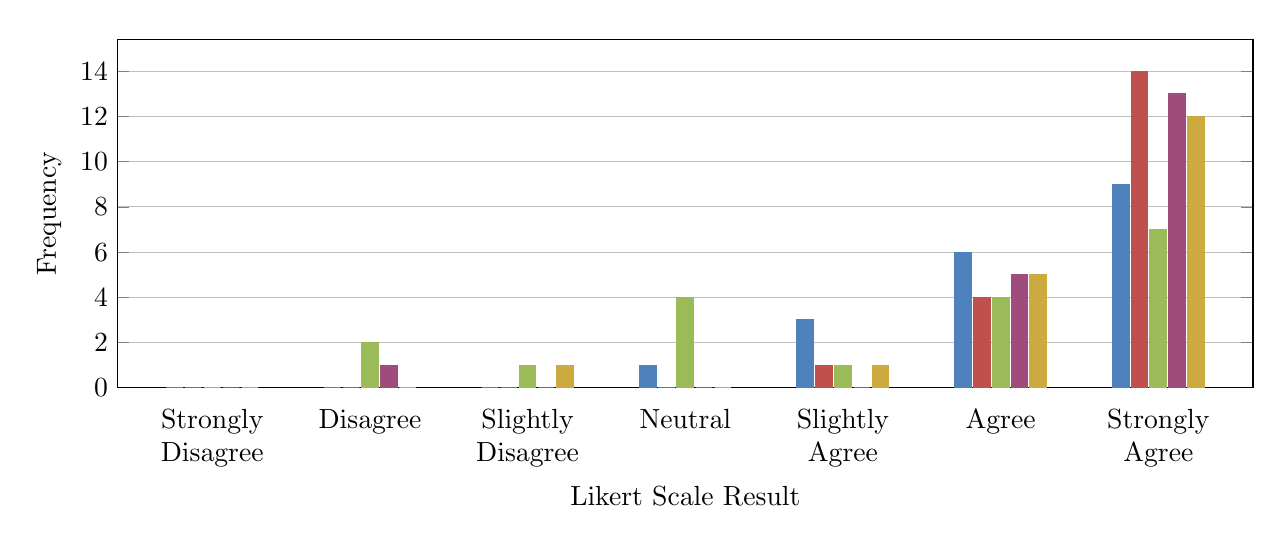
\begin{tikzpicture}
    \begin{axis}[
      % width  = \textwidth,
      width = 16cm,
      height = 6cm,
      major x tick style = transparent,
      ybar=2*\pgflinewidth,
      bar width=6pt,
      ymajorgrids = true,
      ylabel = {Frequency},
      xlabel = {Likert Scale Result},
      symbolic x coords= {-3,-2,-1,0,1,2,3},
      xticklabels = {Strongly Disagree,Disagree,Slightly Disagree,Neutral,Slightly Agree,Agree,Strongly Agree},
      xtick = data,
      ytick = {0,2,4,6,8,10,12,14},
      x tick label style  = {text width=2cm,align=center},
      scaled y ticks = false,
      % enlarge x limits=0.25,
      ymin=0,
      legend cell align=left,
      legend style={
              at={(1,1.05)},
              anchor=south east,
              column sep=1ex
      }
    ]
        \addplot[style={bblue,fill=bblue,mark=none}]
            coordinates {(-3,0) (-2,0) (-1,0) (0,1) (1,3) (2,6) (3,9) };

        \addplot[style={rred,fill=rred,mark=none}]
             coordinates {(-3,0) (-2,0) (-1,0) (0,0) (1,1) (2,4) (3,14) };

        \addplot[style={ggreen,fill=ggreen,mark=none}]
             coordinates {(-3,0) (-2,2) (-1,1) (0,4) (1,1) (2,4) (3,7) };

        \addplot[style={ppurple,fill=ppurple,mark=none}]
             coordinates {(-3,0) (-2,1) (-1,0) (0,0) (1,0) (2,5) (3,13) };

       \addplot[style={yyellow,fill=yyellow,mark=none}]
           coordinates {(-3,0) (-2,0) (-1,1) (0,0) (1,1) (2,5) (3,12) };

        % \legend{It is easier to figure out the turtles path,It is easier to figure out what dynamics different notes are played at,It is easier to tell the order in which dynamics are applied,It is easier to write dynamics in the correct place,Overall system 2 is preferable}
    \end{axis}
\end{tikzpicture}

\subsection{Inferred Octave}

\begin{table}[!htbp]
\centering
% \caption{Grammar rules for turtle movement instructions. $z \in \mathbb{Z}, n \in \mathbb{N}, c \in \texttt{[A-Za-z]}^{+}$.}
\vspace{1pt}
\begin{tabular}{|l|l|l|} \hline
\textbf{Statement}&\textbf{Mode}&\textbf{p-value}\\ \hline
\mycbox{bblue} less effort is required to write a part &Strongly Agree&0.0000 \\ \hline
\mycbox{rred} it is harder to figure out what octave a note will be&Slightly Agree&0.0639 \\
played in&& \\ \hline
\mycbox{ggreen} Overall, system 2 is preferable&Strongly Agree&0.0000 \\ \hline
\end{tabular}
\label{evaluation:inferredOctave}
\end{table}

\vspace{-20pt}
\paragraph{} Depending on its use, the inferred octave notation has the tradeoff that the octave is less easier inferred. There were no strong agreements and only one agreement that this was the case but the modal response was slight agreement. However many users didn't find this an issue and the distribution of responses is not significantly different to uniform. Overall this addition offered a significant improvement.

\vspace{10pt}
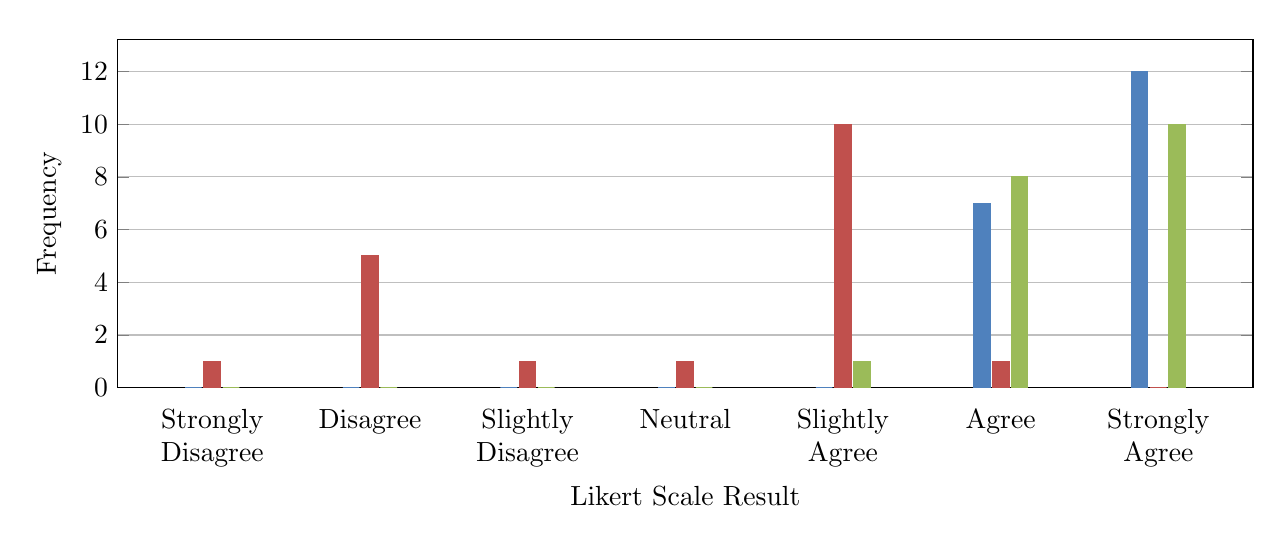
\begin{tikzpicture}
    \begin{axis}[
      width  = 16cm,
      height = 6cm,
      major x tick style = transparent,
      ybar=2*\pgflinewidth,
      bar width=6pt,
      ymajorgrids = true,
      ylabel = {Frequency},
      xlabel = {Likert Scale Result},
      symbolic x coords= {-3,-2,-1,0,1,2,3},
      xticklabels = {Strongly Disagree,Disagree,Slightly Disagree,Neutral,Slightly Agree,Agree,Strongly Agree},
      xtick = data,
      ytick = {0,2,4,6,8,10,12,14},
      x tick label style  = {text width=2cm,align=center},
      scaled y ticks = false,
      % enlarge x limits=0.25,
      ymin=0,
      legend cell align=left,
      legend style={
              at={(1,1.05)},
              anchor=south east,
              column sep=1ex
      }
    ]
    \addplot[style={bblue,fill=bblue,mark=none}]
    	coordinates {(-3,0) (-2,0) (-1,0) (0,0) (1,0) (2,7) (3,12) };
    \addplot[style={rred,fill=rred,mark=none}]
    	coordinates {(-3,1) (-2,5) (-1,1) (0,1) (1,10) (2,1) (3,0) };
    \addplot[style={ggreen,fill=ggreen,mark=none}]
    	coordinates {(-3,0) (-2,0) (-1,0) (0,0) (1,1) (2,8) (3,10) };

    \end{axis}
\end{tikzpicture}

\subsection{Nested Instructions}

\begin{table}[!htbp]
\centering
% \caption{Grammar rules for turtle movement instructions. $z \in \mathbb{Z}, n \in \mathbb{N}, c \in \texttt{[A-Za-z]}^{+}$.}
\vspace{1pt}
\begin{tabular}{|l|l|l|} \hline
\textbf{Statement}&\textbf{Mode}&\textbf{p-value}\\ \hline
\mycbox{bblue} it is easier to parse the turtle instruction and tell &Agree&0.0003\\
what it will do.&& \\ \hline
\mycbox{rred} it is easier to repeat sections of notes.&Strongly Agree&0.0000\\ \hline
\mycbox{ggreen} Overall, system 2 is preferable.&Strongly Agree&0.0000\\ \hline
\end{tabular}
\label{evaluation:nestedInstructions}
\end{table}

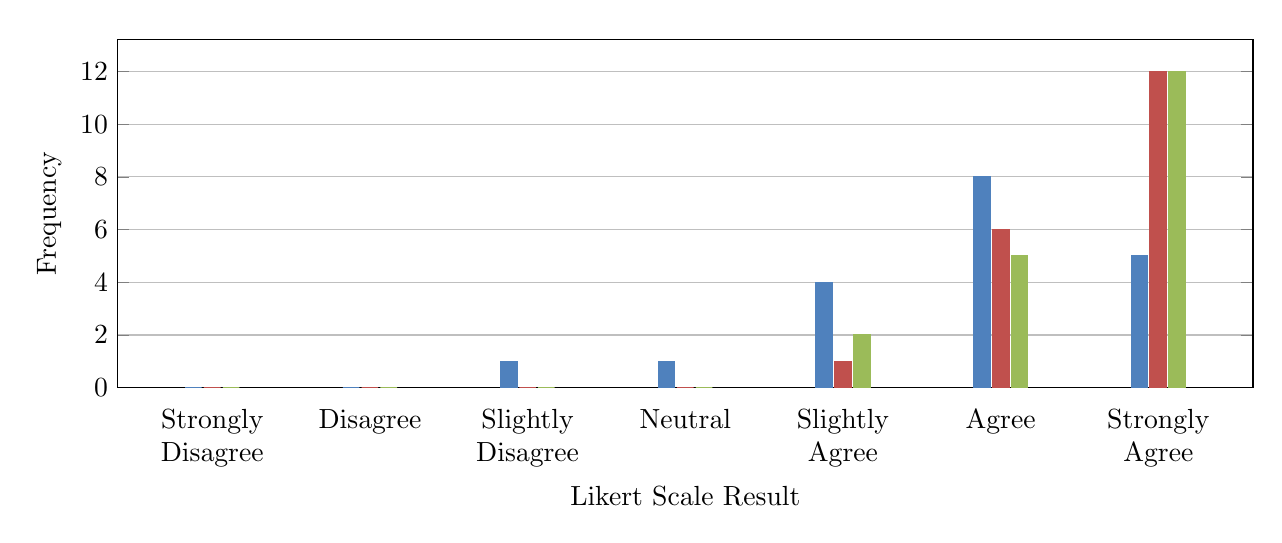
\begin{tikzpicture}
    \begin{axis}[
      % width  = \textwidth,
      width = 16cm,
      height = 6cm,
      major x tick style = transparent,
      ybar=2*\pgflinewidth,
      bar width=6pt,
      ymajorgrids = true,
      ylabel = {Frequency},
      xlabel = {Likert Scale Result},
      symbolic x coords= {-3,-2,-1,0,1,2,3},
      xticklabels = {Strongly Disagree,Disagree,Slightly Disagree,Neutral,Slightly Agree,Agree,Strongly Agree},
      xtick = data,
      ytick = {0,2,4,6,8,10,12,14},
      x tick label style  = {text width=2cm,align=center},
      scaled y ticks = false,
      % enlarge x limits=0.25,
      ymin=0,
      legend cell align=left,
      legend style={
              at={(1,1.05)},
              anchor=south east,
              column sep=1ex
      }
    ]
    \addplot[style={bblue,fill=bblue,mark=none}]
    coordinates {(-3,0) (-2,0) (-1,1) (0,1) (1,4) (2,8) (3,5) };
    \addplot[style={rred,fill=rred,mark=none}]
    coordinates {(-3,0) (-2,0) (-1,0) (0,0) (1,1) (2,6) (3,12) };
    \addplot[style={ggreen,fill=ggreen,mark=none}]
    coordinates {(-3,0) (-2,0) (-1,0) (0,0) (1,2) (2,5) (3,12) };

        % \legend{It is easier to figure out the turtles path,It is easier to figure out what dynamics different notes are played at,It is easier to tell the order in which dynamics are applied,It is easier to write dynamics in the correct place,Overall system 2 is preferable}
    \end{axis}
\end{tikzpicture}

\subsection{Active Turtles}

\begin{table}[!htbp]
\centering
% \caption{Grammar rules for turtle movement instructions. $z \in \mathbb{Z}, n \in \mathbb{N}, c \in \texttt{[A-Za-z]}^{+}$.}
\vspace{1pt}
\begin{tabular}{|l|l|l|} \hline
\textbf{Statement}&\textbf{Mode}&\textbf{p-value}\\ \hline
\mycbox{bblue} it is easier to tell if a certain turtle has been registered.&Strongly Agree&0.0000\\ \hline
\mycbox{rred} it is easier to see where the active turtles are.&(Strongly) Agree&0.0011\\ \hline
\mycbox{ggreen} it is easier to toggle the activation of turtles.in the&Agree&0.0038\\
correct place&& \\ \hline
\mycbox{ppurple} Overall, system 2 is preferable.&Strongly Agree&0.0000 \\ \hline
\end{tabular}
\label{evaluation:activeTurtles}
\end{table}

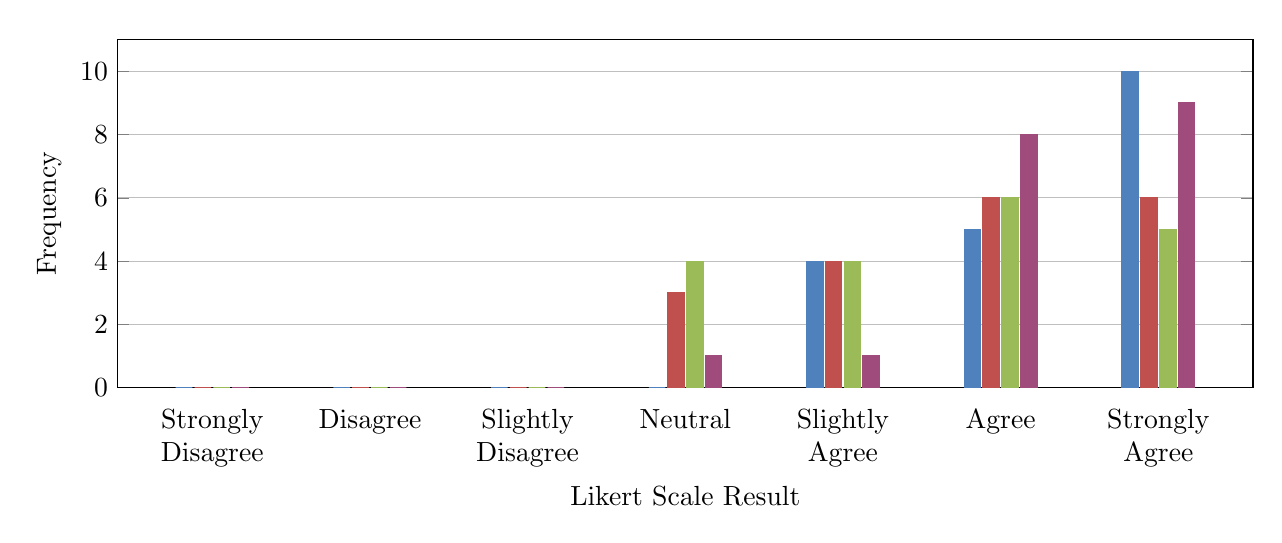
\begin{tikzpicture}
    \begin{axis}[
      % width  = \textwidth,
      width = 16cm,
      height = 6cm,
      major x tick style = transparent,
      ybar=2*\pgflinewidth,
      bar width=6pt,
      ymajorgrids = true,
      ylabel = {Frequency},
      xlabel = {Likert Scale Result},
      symbolic x coords= {-3,-2,-1,0,1,2,3},
      xticklabels = {Strongly Disagree,Disagree,Slightly Disagree,Neutral,Slightly Agree,Agree,Strongly Agree},
      xtick = data,
      ytick = {0,2,4,6,8,10,12,14},
      x tick label style  = {text width=2cm,align=center},
      scaled y ticks = false,
      % enlarge x limits=0.25,
      ymin=0,
      legend cell align=left,
      legend style={
              at={(1,1.05)},
              anchor=south east,
              column sep=1ex
      }
    ]
    \addplot[style={bblue,fill=bblue,mark=none}]
    coordinates {(-3,0) (-2,0) (-1,0) (0,0) (1,4) (2,5) (3,10) };
    \addplot[style={rred,fill=rred,mark=none}]
    coordinates {(-3,0) (-2,0) (-1,0) (0,3) (1,4) (2,6) (3,6) };
    \addplot[style={ggreen,fill=ggreen,mark=none}]
    coordinates {(-3,0) (-2,0) (-1,0) (0,4) (1,4) (2,6) (3,5) };
    \addplot[style={ppurple,fill=ppurple,mark=none}]
    coordinates {(-3,0) (-2,0) (-1,0) (0,1) (1,1) (2,8) (3,9) };

        % \legend{It is easier to figure out the turtles path,It is easier to figure out what dynamics different notes are played at,It is easier to tell the order in which dynamics are applied,It is easier to write dynamics in the correct place,Overall system 2 is preferable}
    \end{axis}
\end{tikzpicture}

\subsection{Continuous Volume}

\begin{table}[!htbp]
\centering
% \caption{Grammar rules for turtle movement instructions. $z \in \mathbb{Z}, n \in \mathbb{N}, c \in \texttt{[A-Za-z]}^{+}$.}
\vspace{1pt}
\begin{tabular}{|l|l|l|} \hline
\textbf{Statement}&\textbf{Mode}&\textbf{p-value}\\ \hline
\mycbox{bblue} it is more intuitive how loud a note will be played.&Disagree&0.6592\\
&Strongly Agree& \\ \hline
\mycbox{rred} the volumes available are less limited.&Strongly Agree&0.0000\\ \hline
\mycbox{ggreen} Overall, system 2 is preferable..&Agree&0.0003\\ \hline
\end{tabular}
\label{evaluation:continuousVolume}
\end{table}

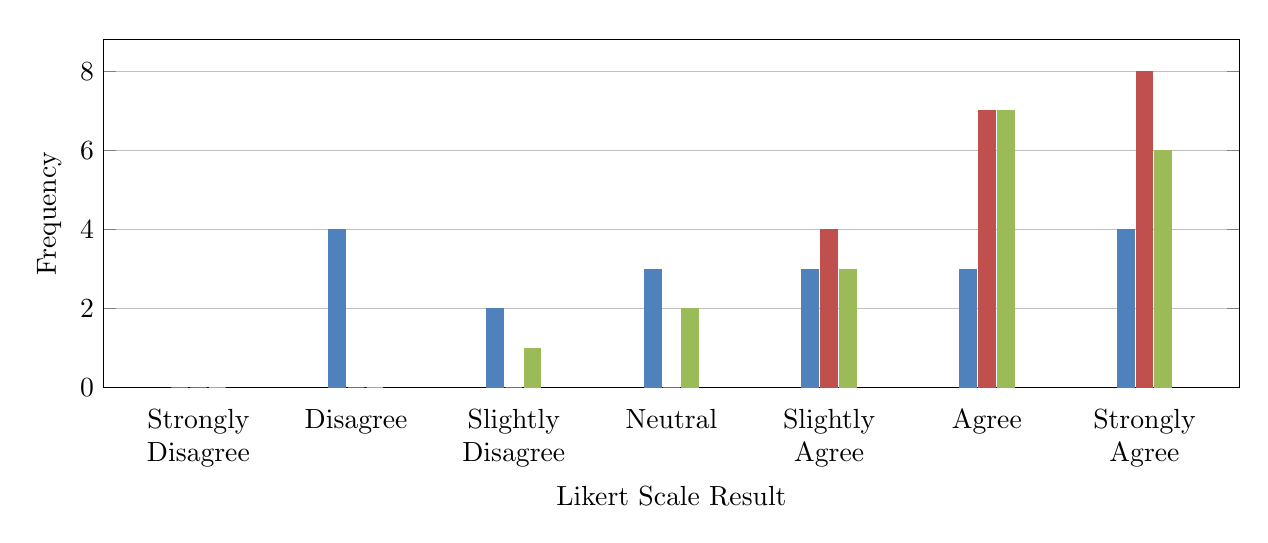
\begin{tikzpicture}
    \begin{axis}[
      % width  = \textwidth,
      width = 16cm,
      height = 6cm,
      major x tick style = transparent,
      ybar=2*\pgflinewidth,
      bar width=6pt,
      ymajorgrids = true,
      ylabel = {Frequency},
      xlabel = {Likert Scale Result},
      symbolic x coords= {-3,-2,-1,0,1,2,3},
      xticklabels = {Strongly Disagree,Disagree,Slightly Disagree,Neutral,Slightly Agree,Agree,Strongly Agree},
      xtick = data,
      ytick = {0,2,4,6,8,10,12,14},
      x tick label style  = {text width=2cm,align=center},
      scaled y ticks = false,
      % enlarge x limits=0.25,
      ymin=0,
      legend cell align=left,
      legend style={
              at={(1,1.05)},
              anchor=south east,
              column sep=1ex
      }
    ]
    \addplot[style={bblue,fill=bblue,mark=none}]
    coordinates {(-3,0) (-2,4) (-1,2) (0,3) (1,3) (2,3) (3,4) };
    \addplot[style={rred,fill=rred,mark=none}]
    coordinates {(-3,0) (-2,0) (-1,0) (0,0) (1,4) (2,7) (3,8) };
    \addplot[style={ggreen,fill=ggreen,mark=none}]
    coordinates {(-3,0) (-2,0) (-1,1) (0,2) (1,3) (2,7) (3,6) };

        % \legend{It is easier to figure out the turtles path,It is easier to figure out what dynamics different notes are played at,It is easier to tell the order in which dynamics are applied,It is easier to write dynamics in the correct place,Overall system 2 is preferable}
    \end{axis}
\end{tikzpicture}

\subsection{Automatic Stepping}

\begin{table}[!htbp]
\centering
% \caption{Grammar rules for turtle movement instructions. $z \in \mathbb{Z}, n \in \mathbb{N}, c \in \texttt{[A-Za-z]}^{+}$.}
\vspace{1pt}
\begin{tabular}{|l|l|l|} \hline
\textbf{Statement}&\textbf{Mode}&\textbf{p-value}\\ \hline
\mycbox{bblue} less mental work is required to write the turtle &Strongly Agree&0.0000\\
instructions.&& \\ \hline
\mycbox{rred} less work is required when more notes wish to be added.&Strongly Agree&0.0000\\ \hline
\mycbox{ggreen} Overall, system 2 is preferable.&Strongly Agree&0.0000\\ \hline
\end{tabular}
\label{evaluation:automaticStepping}
\end{table}

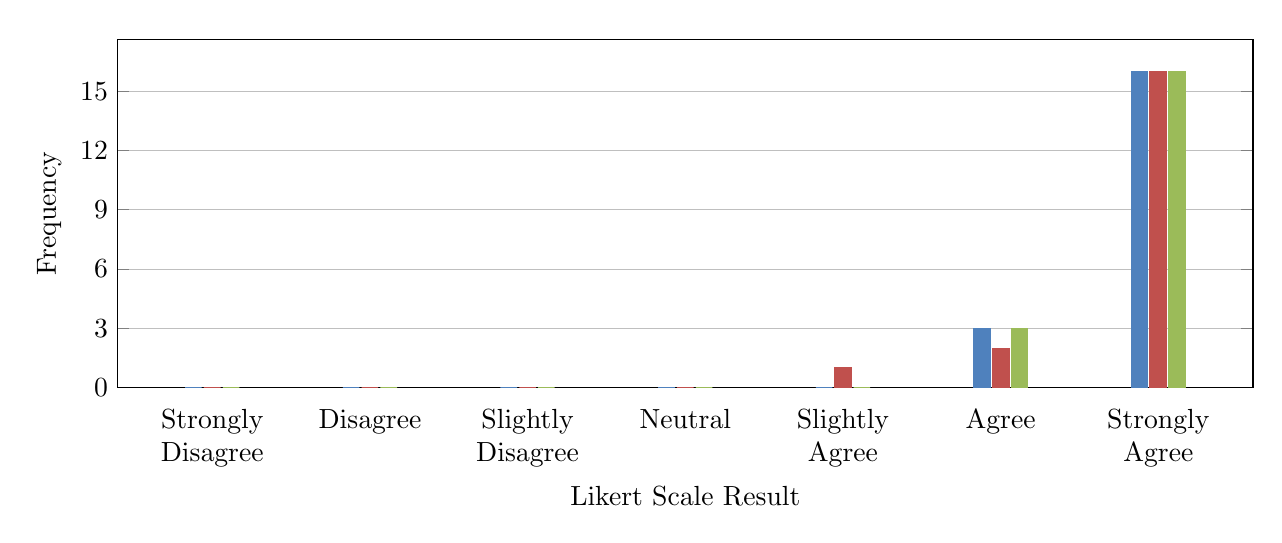
\begin{tikzpicture}
    \begin{axis}[
      % width  = \textwidth,
      width = 16cm,
      height = 6cm,
      major x tick style = transparent,
      ybar=2*\pgflinewidth,
      bar width=6pt,
      ymajorgrids = true,
      ylabel = {Frequency},
      xlabel = {Likert Scale Result},
      symbolic x coords= {-3,-2,-1,0,1,2,3},
      xticklabels = {Strongly Disagree,Disagree,Slightly Disagree,Neutral,Slightly Agree,Agree,Strongly Agree},
      xtick = data,
      ytick = {0,3,6,9,12,15},
      x tick label style  = {text width=2cm,align=center},
      scaled y ticks = false,
      % enlarge x limits=0.25,
      ymin=0,
      legend cell align=left,
      legend style={
              at={(1,1.05)},
              anchor=south east,
              column sep=1ex
      }
    ]
    \addplot[style={bblue,fill=bblue,mark=none}]
    coordinates {(-3,0) (-2,0) (-1,0) (0,0) (1,0) (2,3) (3,16) };
    \addplot[style={rred,fill=rred,mark=none}]
    coordinates {(-3,0) (-2,0) (-1,0) (0,0) (1,1) (2,2) (3,16) };
    \addplot[style={ggreen,fill=ggreen,mark=none}]
    coordinates {(-3,0) (-2,0) (-1,0) (0,0) (1,0) (2,3) (3,16) };

        % \legend{It is easier to figure out the turtles path,It is easier to figure out what dynamics different notes are played at,It is easier to tell the order in which dynamics are applied,It is easier to write dynamics in the correct place,Overall system 2 is preferable}
    \end{axis}
\end{tikzpicture}

\subsection{Absolute Tempo}

\begin{table}[!htbp]
\centering
% \caption{Grammar rules for turtle movement instructions. $z \in \mathbb{Z}, n \in \mathbb{N}, c \in \texttt{[A-Za-z]}^{+}$.}
\vspace{1pt}
\begin{tabular}{|l|l|l|} \hline
\textbf{Statement}&\textbf{Mode}&\textbf{p-value}\\ \hline
\mycbox{bblue} it is easier to tell what the speed instruction&Strongly Agree&0.0000\\
 corresponds to&& \\ \hline
\mycbox{rred} giving an exact tempo (e.g. when transcribing sheet&Strongly Agree&0.0000\\
music) is easier&& \\ \hline
\mycbox{ggreen} Overall, system 2 is preferable.&Strongly Agree&0.0000\\ \hline
\end{tabular}
\label{evaluation:absoluteTempo}
\end{table}

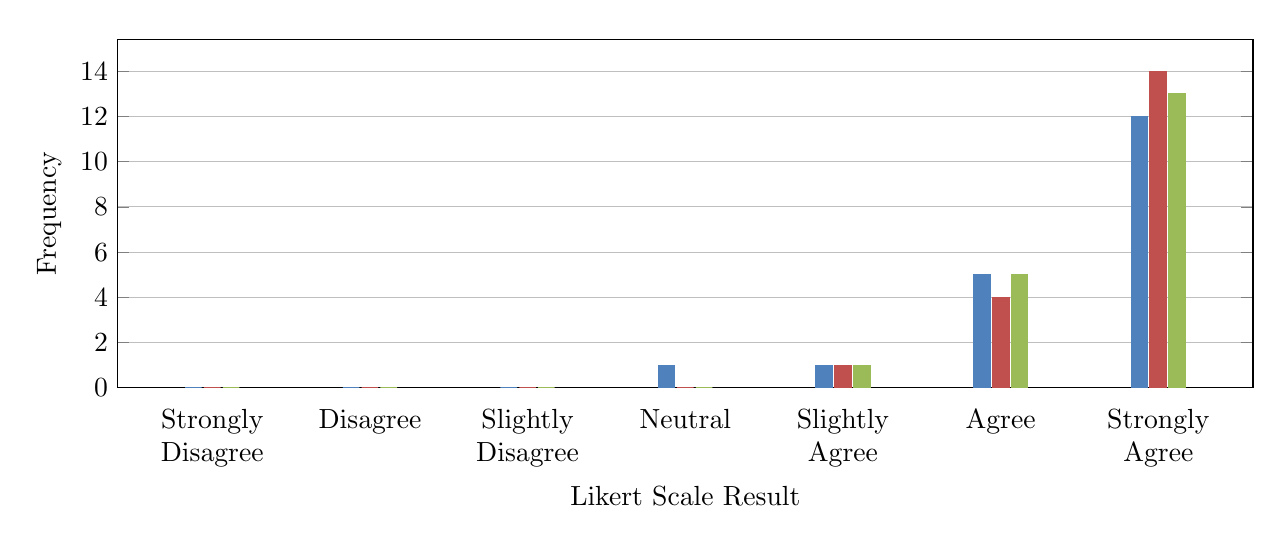
\begin{tikzpicture}
    \begin{axis}[
      % width  = \textwidth,
      width = 16cm,
      height = 6cm,
      major x tick style = transparent,
      ybar=2*\pgflinewidth,
      bar width=6pt,
      ymajorgrids = true,
      ylabel = {Frequency},
      xlabel = {Likert Scale Result},
      symbolic x coords= {-3,-2,-1,0,1,2,3},
      xticklabels = {Strongly Disagree,Disagree,Slightly Disagree,Neutral,Slightly Agree,Agree,Strongly Agree},
      xtick = data,
      ytick = {0,2,4,6,8,10,12,14},
      x tick label style  = {text width=2cm,align=center},
      scaled y ticks = false,
      % enlarge x limits=0.25,
      ymin=0,
      legend cell align=left,
      legend style={
              at={(1,1.05)},
              anchor=south east,
              column sep=1ex
      }
    ]
    \addplot[style={bblue,fill=bblue,mark=none}]
    coordinates {(-3,0) (-2,0) (-1,0) (0,1) (1,1) (2,5) (3,12) };
    \addplot[style={rred,fill=rred,mark=none}]
    coordinates {(-3,0) (-2,0) (-1,0) (0,0) (1,1) (2,4) (3,14) };
    \addplot[style={ggreen,fill=ggreen,mark=none}]
    coordinates {(-3,0) (-2,0) (-1,0) (0,0) (1,1) (2,5) (3,13) };

        % \legend{It is easier to figure out the turtles path,It is easier to figure out what dynamics different notes are played at,It is easier to tell the order in which dynamics are applied,It is easier to write dynamics in the correct place,Overall system 2 is preferable}
    \end{axis}
\end{tikzpicture}
